%% The following is a directive for TeXShop to indicate the main file
%%!TEX root = diss.tex
\chapter{Deconvolution of mixed signals via structured optimization}
\label{ch:App-Sig-Demix}

\section{Introduction} 

The signal demixing problem seeks to separate a superposition of signals into its constituent components. In the measurement model we consider, a set of signals $\{x\nai\}_{i=1}^k$ in $\Re^n$ are observed through noisy
measurements $b\in\Re^m$, with $m\le n$, of the form
\begin{equation}\label{eq:demixing-problem}
  b = M\xagg + \eta \text{with} \xagg\coloneqq \sum\limits_{i = 1}^k x\nai.
\end{equation}
The known linear operator $M:\Re^n \rightarrow \Re^m$ models the acquisition process of the superposition vector $\xagg$. The vector $\eta\in \Re^m$ represents noise uncorrelated with the data. This measurement model and its variations are useful for a range of data-science applications, including mixture models~\citep{araki2009blind,quiros2012dependent}, blind deconvolution~\citep{ahmed2013blind}, blind source separation~\citep{chan2008convex}, and morphological component analysis~\citep{bobin2007morphological}.

A central concern of the demixing problem \eqref{eq:demixing-problem} is to delineate efficient procedures and accompanying conditions that make it possible to recover the constituent signals to within a prescribed accuracy---using the fewest number of measurements $m$. The recovery of these constituent signals cannot be accomplished without additional information, such as the latent structure in each signal $x\nai$. We build on the general atomic-sparsity framework introduced in \autoref{sec:1-3}, namely each signal $x\nai$ is itself well represented as a superposition of a few atomic signals from a collection  $\Ascr_i\subset\Re^n$. In other words, the vectors $\{x\nai\}_{i=1}^k$ are paired with atomic sets $\{\Ascr_i\}_{i=1}^k$ that allow the decompositions
\begin{equation} \label{eq:decomposition}
  x\nai = \sum_{a\in \Ascr_i}c_a a, \quad c_a\geq 0\quad \forall a \in \Ascr_i,
\end{equation}
where most of the coefficients $c_a$ are zero.

As we introduced in \autoref{ch:Dual-Struc-Opt}, a common approach to recover an atomic-sparse signal is to use the gauge function \eqref{eq:gauge1}. The typical approach to the demixing problem is to combine $k$ separate gauge functions, each corresponding to one of the atomic sets $\{\Ascr_i\}_{i=1}^k$, as a weighted sum or similar formulations. We instead combine the $k$ separate gauge functions using a special-purpose convolution operation called polar convolution, that can reflect the additive structure of the superposition, as defined in~\eqref{eq:demixing-problem}.

\subsection{Polar convolution} \label{sec:3-1-1}

Recall that for any two atomic sets $\Ascr_1$ and $\Ascr_2$, the polar convolution of the corresponding gauge functions is given by \eqref{eq:max-conv}.
The resulting function is the gauge to the vector sum $\Ascr_1+\Ascr_2$, i.e.,
\begin{equation}\label{eq-polar-convolution-sum}
  \gauge\Aso\maxconv\gauge\Ast = \gauge_{\scriptscriptstyle\Ascr_1+\Ascr_2};
\end{equation}
cf. \autoref{prop:max-convolution}. 

\begin{figure}[t]
    \centering
    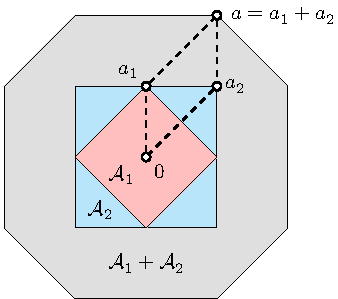
\includegraphics[page=1]{./figures/illustrations2.pdf}
    \caption{The sum of two atomic sets. The sum \(\Ascr_1+\Ascr_2\) is the unit level set for the polar convolution $\gauge\Aso\maxconv\gauge\Ast$, i.e., $\Ascr_1+\Ascr_2 = \{a \mid \gauge\Aso\maxconv\gauge\Ast(a) \leq 1\}$.\label{fig:sum-sets}}
\end{figure}

The subdifferential properties of polar convolution facilitate our analysis and allow us to build an efficient algorithm that is practical for a range of problems. In particular, the polar convolution decouples under a duality correspondence built around the polarity of convex sets. Under such duality correspondence,
\[
  \gauge_{\scriptscriptstyle(\Ascr_1+\Ascr_2)\polar}
  = \gauge_{\scriptscriptstyle\Ascr_1\polar} + \gauge_{\scriptscriptstyle\Ascr_2\polar},
\]
which implies that the subdifferential decouples as 
$\partial \gauge_{\scriptscriptstyle(\Ascr_1+\Ascr_2)\polar} = \partial\gauge_{\scriptscriptstyle\Ascr_1\polar}+\partial\gauge_{\scriptscriptstyle\Ascr_2\polar}$. Thus, a subgradient computation, which is central to all first-order methods for convex optimization, can be implemented using only subdifferential oracles for each of the polar functions $\gauge_{\scriptscriptstyle\Ascr_i\polar}$. 

\subsection{Decompression and deconvolution} \label{sec:3-1-2}

The principle innovation of our approach to the demixing problem \eqref{eq:demixing-problem} is to decouple the recovery procedure into two stages: an initial \emph{decompression} stage meant to recover the superposition $\xagg$ from the vector of observations $b$, followed by a \emph{deconvolution} stage that separates the recovered superposition $\xagg$ into its constituent components $\{x\nai\}_{i=1}^k$. We couple the convex theory of polar convolution~\citep{friedlander2019polarconvolution} to the theory of statistical dimension and signal incoherence to derive a recovery procedure and analysis for demixing a compressively sampled mixture to within a prescribed accuracy.

\paragraph{Stage 1: Decompression} The initial decompression stage is based on the observation
that because each signal $x\nai$ is $\Ascr_i$ sparse, the superposition $\xagg$
must be sparse with respect to the weighted vector sum
\begin{equation} \label{eq:weighted-atomic-sum}
  \Ascr\subs\coloneqq\sum_{i=1}^k\lambda_i\Ascr_i
  ~\equiv \left\{\sum_{i=1}^k\lambda_ia_i ~\bigg\vert~ a_i\in\Ascr_i\cup\{0\},\ i\in\irange1k\right\}
\end{equation}
of the individual atomic sets $\Ascr_i$. The positive weights $\lambda_i$ carry information about the relative powers of the individual signals, and serve to equilibrate the gauge values of each signal. Thus, the weights $\lambda_i$ are defined so that for each $i\in\irange1k$,
\begin{equation}\label{eq-lambda-def}
  \gauge_{\scriptscriptstyle\lambda_i\Ascr_i}(x\nai)=\gauge\Aso(x\nao). 
\end{equation}
The initial decompression stage solves the convex optimization problem
\begin{equation} \tag{P1} \label{eq:decompression}
  \minimize{x\in\Re^n}\enspace \gauge\Ass(x) \enspace\st\enspace \|Mx - b\|_2 \leq \alpha,
\end{equation}
where the parameter $\alpha\ge0$ bounds the acceptable level of misfit between the linear model \(Mx\) and the observations $b$, and correspondingly reflects the anticipated magnitude of the noise $\eta$. It follows from~\eqref{eq-polar-convolution-sum} that the objective of \eqref{eq:decompression} is in fact the polar convolution of the individual weighted gauges:
\begin{equation*}
   \gauge_{\scriptscriptstyle\Ascr\subs}(x)
   = \gauge_{\scriptscriptstyle\lambda_1\Ascr_1}\maxconv\gauge_{\scriptscriptstyle\lambda_2\Ascr_2}\maxconv\cdots\ \maxconv\gauge_{\scriptscriptstyle\lambda_k\Ascr_k}(x).
\end{equation*}
\autoref{thm-stability} establishes conditions under which the solution $x\subs^*$ to~\eqref{eq:decompression} stably approximates the superposition $\xagg$.

\paragraph{Stage 2: Deconvolution} The solution $x\subs^*$ of the decompression problem \eqref{eq:decompression} defines the subsequent convex deconvolution problem
\begin{equation} \tag{P2} \label{eq:deconvolution}
  \minimize{x_1, \ldots, x_k}
  \enspace \max_{i\in1:k}\, \gauge_{\scriptscriptstyle\lambda_i\Ascr_i}(x_i)
  \enspace\st\enspace
  \textstyle\sum_{i = 1}^k x_i = x\subs^*
\end{equation}
to obtain approximations $x_i^*$ to each constituent signal $x\nai$. 

In both stages, a variant of the conditional-gradient method provides a
computationally and memory efficient algorithm that can be implemented with
storage proportional to the number of measurements $m$~\citep{fan2019alignment}. We
describe in \autoref{ch:App-AtomicOpt} the details of the method.

\subsection{Related work}

\begin{table}[t]
  \begin{center}
  \begin{tabular}{lc@{\enspace}c@{\enspace}c@{\enspace}c@{\enspace}c} 
  \toprule
            & Compressed   & Noisy        & Number& Recovery  & Explicit \\
  Reference & measurements & observations & of signals  & algorithm & error bound\\\midrule
  \citep{mccoy2014convexity} & \xmark & \xmark & $2$  &\cmark  &\xmark\\
  \citep{mccoy2014sharp} & \xmark & \xmark & $2$ & \xmark & \cmark \\
  \citep{oymak2017universality} & \cmark & \xmark & $2$ &\xmark & \cmark \\
  \citep{mccoy2013achievable} & \cmark & \cmark & $\geq 2$ &\xmark & \xmark \\
  \autoref{ch:App-Sig-Demix} & \cmark & \cmark & $\geq 2$ & \cmark & \cmark \\\bottomrule 
  \end{tabular}
  \end{center}
  \caption{Comparison of the main mathematical results obtained by \autoref{ch:App-Sig-Demix} and related references. Only \autoref{ch:App-Sig-Demix} and~\citet{mccoy2013achievable} consider the case of two or more signals.} \label{tab:comparasion}
\end{table}

The history of signal demixing can be traced to early work in seismic imaging~\citep{claerbout1973robust} and morphological component analysis~\citep{starck2005morphological,bobin2007morphological}, which used 1-norm regularization to separate incoherent signals. More recently,~\citet{mccoy2014sharp,mccoy2013achievable} and \citet{oymak2017universality} proposed a unified theoretical framework for signal demixing using modern tools from high-dimensional geometry.

\citet{mccoy2014convexity} analyzed the recovery guarantees of a convex program that can reconstruct $k = 2$ randomly-rotated signals from a full set of noiseless observations, i.e., $M$ is the identity matrix and $\norm{\eta}=0$. They also provided an ADMM-type algorithm for solving their proposed model. \citet{mccoy2014sharp} enhanced the error bound analysis under the same problem setting. \citet{mccoy2013achievable} subsequently extended this framework to demixing $k \geq 2$ randomly-rotated signals from noisy measurements, as modeled by~\eqref{eq:demixing-problem}. However, the constants in the recovery error bound are not made explicit. We postpone to \autoref{sec:comparasion} a detailed comparison between our theoretical results and theirs. \citet{oymak2017universality} considered a demixing problem similar to~\eqref{eq:deconvolution} that also incorporates the measurement operator $M$, and provided guarantees for demixing two unknown vectors from random and noiseless measurements. We build on this line of work by providing explicit recovery error bounds in terms of the complexity of the signal sets and the number of measurements. Our analysis allows for any number of individual signals $k\ge2$. Moreover, we provide a memory-efficient algorithm for solving our proposed model. \autoref{tab:comparasion} compares main mathematical results obtained by \autoref{ch:App-Sig-Demix} and the above references.

Early work on demixing sparse signals implicitly assumed some notion of incoherence between representations of the signals. This concept was made concrete by \citet{doh01}, and subsequently \citet{doe03}, who measured the mutual incoherence of finite bases via the maximal inner-products between elements of the sets. Related incoherence definitions appear in compressed sensing~\citep{tro04, maleki2009coherence} and robust PCA~\citep{candes2011robust, wright2013compressive}. In this chapter we adopt \citet{mccoy2013achievable}'s notion of incoherence as the minimal angle between conic representation of the individual signals.

\subsection{Roadmap}

\autoref{sec:3-2} shows that the decompression problem \eqref{eq:decompression} can stably recover $x\nag$. \autoref{thm:tropp} characterizes the recovery error in terms of the overall complexity of the signal, provided the measurements are random. This result follows directly from \citet{tropp2015convex} and a conic decomposition property particular to polar convolution. \autoref{sec:3-3} shows that the deconvolution problem~\eqref{eq:deconvolution} can stably approximate each $x\nai$. The bound in the recovery error is given in terms of the error in the initial decompression process and the incoherence between signals as measured by the minimum angle between conic representations of each signal; see \autoref{thm-stability}. This result requires a general notion of incoherence based on the angle between descent cones, first analyzed by \citet{mccoy2013achievable}.  \autoref{sec-incoherence} shows how a random-rotation model yields a particular level of incoherence with high probability; see \autoref{thm:Incoherence}. We develop the recovery guarantee under the random-rotation model; see \autoref{corollary-stability}. \autoref{sec:3-5} describes experiments on real and synthetic structured signals. Proofs of all theoretical results are given in \autoref{sec:3-7}.

The following blanket assumption holds throughout this chapter.
\begin{assumption}[Measurement model]\label{assume-blanket}
  The linear model~\eqref{eq:demixing-problem} satisfies the following conditions: the linear map
  $M:\Re^n\to\Re^m$ has i.i.d.\@ standard Gaussian entries; the noise vector $\eta$ satisfies $\|\eta\|_2\leq \alpha$ for some scalar $\alpha$; and the relative signal powers $\{\lambda_i\}_{i=1}^k$ satisfy~\eqref{eq-lambda-def}.
\end{assumption} 

\subsection{Summary of contributions}\label{sec:3-6}

In this chapter, we study the structural signal demixing problem. We develop a two-stage, decompression-deconvolution approach for compressed signal demixing motivated by the polar convolution of gauge functions and the polar alignment property developed in \autoref{ch:Dual-Struc-Opt}. Under the assumption of Gaussian measurements and randomly rotated signals, we develop explicit signal-recovery error and sample complexity bounds for the two-stage approach. These are the first known explicit error bounds for recovering an arbitrary number of mixed and compressed signals. Extensive numerical experiments on synthetic and real data verify the correctness of our theoretical results and the effectiveness of our approach.


\section{Decompressing the superposition}\label{sec:3-2} 

\begin{figure}[t]
    \centering
   \includegraphics[page=7]{./figures/illustrations2} 
  \caption{A non-trivial intersection of $\Dscr(\Ascr, x\na)$ and $\Null(M)$ is required for successful decompression. The blue shaded region represents the shifted descent cone $x\na + \Dscr(\Ascr, x\na)$, and red line represents the shifted null space $\Null(M) + x\na$. If $\Dscr(\Ascr, x\na) \cap \Null(M) \neq \{0\}$ (as depicted here) then there exists a vector $\hat x$ such that  $\gauge\As(\hat x) < \gauge\As(x\na)$ and $M\hat x = Mx\na$.\label{fig:descent-cone}}
\end{figure}

As shown in \autoref{sec:3-1-2}, under the assumption that the individual signals $x\nai$ are $\Ascr_i$ sparse, the aggregate signal $\xagg$ is sparse with respect to the aggregate atomic set $\Ascr\subs$.
Thus, the decompression of the observations $b$ in \eqref{eq:demixing-problem} is accomplished by minimizing the gauge to $\Ascr\subs$ to within the bound on the noise level $\|\eta\|_2\le\alpha$, as modeled by the recovery problem \eqref{eq:decompression}.
Without noise (i.e., $\alpha=0$), the aggregate signal $\xagg$ is the unique solution to \eqref{eq:decompression} when the null space of the measurement operator $M$ has only a trivial intersection with the descent cone $\Dscr\subs\coloneqq\Dscr(\Ascr\subs, \xagg)$.
In other words, $\xagg$ is the unique solution of \eqref{eq:decompression} if and only if 
\begin{equation}\label{eq-unique-optimality}
  \Dscr\subs\cap\Null(M) = \{0\}.  
\end{equation}
\autoref{fig:descent-cone} illustrates the geometry of this optimality condition, and depicts a case in which it doesn't hold.

If the linear operator $M$ is derived from Gaussian measurements, \citet{gordon1988milman} characterized the probability of the event~\eqref{eq-unique-optimality} as a function of the Gaussian width of the descent cone $\Dscr\subs$ and the number of measurements $m$. This result is the basis for recovery guarantees developed by \citet{chandrasekaran2012convex} and \citet{tropp2015convex} for a convex formulation similar to \eqref{eq:decompression}.

Intuitively, the number of measurements required for stable recovery of the aggregate $\xagg$ depends on the total complexity of the $k$ constituent $\Ascr_i$-sparse vectors $x\nai$. The complexity is measured in terms of the statistical dimension of each of the descent cones $\Dscr_i$.
\citet{tropp2015convex} established a bound on the recovery error between the solutions of the decompression problem~\eqref{eq:decompression} and the superposition $x\nag$ that depends on the statistical dimension $\delta(\Dscr\subs)$ of its descent cone. The following proposition is a restatement of \citep[Corollary~3.5]{tropp2015convex} applied to the decompression problem \eqref{eq:decompression}.

\begin{proposition}[Stable decompression of the aggregate]%
    \label{thm:tropp}
    For any $t>0$, any solution $x^*$ of \eqref{eq:decompression} satisfies
    \begin{equation*}
        \|x^* - \xagg\|_2 \leq 2\alpha\left[\sqrt{m - 1} - \sqrt{\delta(\Dscr\subs)} - t\right]_+^{-1}
    \end{equation*}
    with probability at least $1 - \exp(-t^2/2)$, where $[\xi]_+=\max\{0,\xi\}$. 
\end{proposition}

The statistical dimension of $\Dscr\subs$ is in general challenging to compute. However, we show in \autoref{sec:3-3-1} that when all the signals $\{x\nai\}_{i=1}^k$ are incoherent, a reasonable upper bound on $\delta(\Dscr\subs)$ can be guaranteed; see \autoref{coro:bound_sta_dim}.

As we can see from~\autoref{thm:tropp}, the recovery error bound has a linear dependence with the noise level $\alpha$. This result relies on the assumption that the noise level is over-estimated, i.e. $\alpha \geq \|\eta\|_2$; see~\autoref{assume-blanket}. However, when the noise level is under-estimated, i.e., $\alpha < \|\eta\|_2$, we can not provide any meaningful recovery error bound. This discussion suggests that if in practice, we don't know the true noise level, then we can start with a relative large $\alpha$, and keep reducing it until we get some reasonably good results.

\section{Deconvolving the components}\label{sec:3-3}

The second stage of our approach is the deconvolution stage which separates the recovered aggregate signal into its constituent components. In order to successfully separate the aggregate $x\nag$ into its components $\{x\nai\}_{i=1}^k$ using the deconvolution problem \eqref{eq:deconvolution}, additional assumption on dissimilarity between the atomic representations of the individual signals is generally required. For example, it can be challenging to separate the superposition of two sparse signals or two low-rank signals without additional assumptions. We follow \citet{mccoy2013achievable}, and measure the dissimilarity between signal structures---and thus their incoherence---using the angles between corresponding descent cones.

\begin{figure}[t]
    \centering
    \begin{tabular}{@{}cccc@{}}
      \includegraphics[width=.22\textwidth, page=3]{./figures/illustrations2}
    & \includegraphics[width=.22\textwidth, page=4]{./figures/illustrations2}
    & \includegraphics[width=.22\textwidth, page=5]{./figures/illustrations2}
    & \includegraphics[width=.22\textwidth, page=6]{./figures/illustrations2}
  \\ (a) \small $\Dscr_1\coloneqq\Dscr(\Ascr_1, x_1\na)$ & (b) \small  $\Dscr_2\coloneqq\Dscr(\Ascr_2, x_2\na)$ & (c) \small $d \in -\Dscr_1\cap\Dscr_2$ & (d) \small $x_1\na - d$ and $x_2\na + d$ 
    \end{tabular}
    \caption{The top row depicts two scaled atomic sets $\gauge\Aso(x_i\na)\cdot\Ascr_i$ and the corresponding descent cones $x_i\na + \Dscr_i$ (shifted to lie at $x_i\na$) for $i=1,2$. (c) The descent cones shifted to $x\na = x_1\na + x_2\na$, with $\Dscr_1$ negated; the vector $d$ lies in their intersection. (d) The vector $d$ descends on both scaled atomic sets, so that $\gauge\Aso(x_1\na - d) < \gauge\Aso(x_1)$ and $\gauge\Ast(x_2\na + d) < \gauge\Ast(x_2\na)$.}
    \label{fig:angle_cone}
\end{figure}

To motivate the incoherence definition, consider the case where there are only $k=2$ signals $x\nao$ and $x\nat$. If the descent cones $-\Dscr_1$ and $\Dscr_2$ have a nontrivial intersection, then there exists a nonzero direction $d \in -\Dscr_1 \cap \Dscr_2$ such that $\gauge\Aso(x\nao - d)<\gauge\Aso(x\nao)$ and $\gauge\Ast(x\nat + d)<\gauge\Ast(x\nat)$, which contradicts the optimality condition required for $x\nao$ and $x\nat$ to be unique minimizers of \eqref{eq:deconvolution}.  Thus, deconvolution only succeeds if the descent cones have a trivial intersection, which can be characterized using angle between the descent cones. \autoref{fig:angle_cone} illustrates this geometry. 

\citet{obert1991angle} defined the angle between two cones $\Kscr_1$ and $\Kscr_2$ in $\Re^n$ as the minimal angle between vectors in these two cones. It follows that the cosine of the angle between two cones can be expressed as 
\begin{equation*}
\cos\angle(\Kscr_1, \Kscr_2) 
= \sup\left\{\ip{x}{y} \mid x \in \Kscr_1\cap\mS^{n - 1},\, y \in \Kscr_2\cap\mS^{n - 1}\right\}.
\end{equation*}
For the general case where the number of signals $k\ge2$, a natural choice for a measure of incoherence between these structured signals is the minimum angle between the descent cone of a signal with respect to the remaining descent cones. 

\begin{definition} \label{def:incoherence}
    The pairs $\{(x\nai, \Ascr_i)\}_{i=1}^k$ are $\beta$-incoherent with $\beta\in(0,1]$ if for all $i\in\irange1k$,
    \[
        \cos\angle\left({-\Dscr_i},\, \sum_{j \neq i}\Dscr_j\right)
        \leq 1 - \beta. 
    \]
\end{definition}

We use the incoherence between descent cones to bound the error between the true constituent signals $\{x\nai\}_{i=1}^k$ and the solution set of the deconvolution problem~\eqref{eq:deconvolution}. This bound depends on the accuracy of the approximation $x\subs^*$ to the true superposition $x\nag$ and is shown in \autoref{thm-stability}.

\begin{proposition}[Stable deconvolution]\label{thm-stability} 
    If the pairs $\{(x\nai, \Ascr_i)\}_{i=1}^k$ are $\beta$-incoherent for some $\beta\in(0,1]$, then any set of solutions $\{x_i^*\}_{i=1}^k$ of~\eqref{eq:deconvolution} satisfies for all $i\in\irange1k$
    \begin{align*}
        \|x_i^* - x\nai\|_2 \leq \|x\subs^*-\xagg\|_2/\sqrt{\beta},
    \end{align*}
    where $x\subs^*$ is any solution of~\eqref{eq:decompression}.
\end{proposition}

In summary, a large angle between negation of a descent cone $-\Dscr_i$ and all the other descent cones---as reflected by a large incoherence constant $\beta$---corresponds a small error between each $x_i^*$ and the ground truth $x\nai$.

\subsection{Bound on \texorpdfstring{$\delta(\Dscr\subs)$}{Ds} under incoherence}\label{sec:3-3-1}

\autoref{thm:tropp} gives a stable recovery result for the decompression stage. However, the recovery bound depends on the the statistical dimension of $\Dscr\subs$, which is challenging to compute even when the statistical dimension of the individual descent cone $\Dscr_i$ is known. In this section, we show that the incoherence between the structured signals $\{x\nai\}_{i=1}^k$ is sufficient to establish an upper bound for $\delta(\Dscr\subs)$. 
We start with the $k = 2$ case. \autoref{prop:bound_sta_dim} shows that if the angle between two cones is bounded, then the statistical dimension of the sum of these two cones is also bounded. 

\begin{proposition}[Bound on statistical dimension of sum]\label{prop:bound_sta_dim}
    Let $\Kscr_1$ and $\Kscr_2$ be two closed convex cones in $\Re^n$. If $\cos\angle(-\Kscr_1, \Kscr_2) \leq 1 - \beta$ for some $\beta \in (0, 1]$, then 
    \[\sqrt{\delta(\Kscr_1 + \Kscr_2)} \leq \tfrac{1}{\sqrt{\beta}}\left(\sqrt{\delta(\Kscr_1)} + \sqrt{\delta(\Kscr_2)} \right).\]
\end{proposition}

This result generalizes to an arbitrary number of cones. 
\begin{corollary}[Bound on statistical dimension of sum under incoherence]\label{coro:bound_sta_dim}
   If the pairs $\{(x\nai, \Ascr_i)\}_{i=1}^k$ are $\beta$-incoherent for some $\beta\in(0,1]$, then
   \[\sqrt{\delta(\Dscr\subs)} \leq \beta^{-\tfrac{k-1}{2}}\sum_{i=1}^k\sqrt{\delta(\Dscr_i)}.\]
\end{corollary} 
\autoref{coro:bound_sta_dim} shows that when the pairs $\{(x\nai, \Ascr_i)\}_{i=1}^k$ are $\beta$-incoherent, $\delta(\Dscr\subs)$ can be upper bounded in terms of the statistical dimension of individual descent cones.

\section{Inducing incoherence through random rotation}\label{sec-incoherence}

\autoref{thm-stability} establishes the stability of the deconvolution problem in the case that the unknown signals are $\beta$-incoherent, as formalized in \autoref{def:incoherence}. However, except in very special cases like randomly rotated signals, it is not feasible to determine the incoherence constant $\beta$. We build on McCoy and Tropp's random rotation model~\citep{mccoy2013achievable} to quantify, with high probability, the $\beta$-incoherence of $k$ randomly-rotated atomic sparse signals, and present a recovery result for a randomly rotated case.

We first consider a simpler case of two general cones, one of which is randomly rotated. Let $\SO(n)$ denote the special orthogonal group, which consists of all $n$-by-$n$ orthogonal matrices with unit determinant. The following proposition provides a probabilistic bound on the angle between the two cones in terms of their statistical dimension. This geometric result maybe of intrinsic interest in other contexts.

\begin{proposition}[Probabilistic bound under random rotation] \label{prop-angle-cones}
    Let $Q$ is drawn uniformly at random from $\SO(n)$. Let $\Kscr_1$ and $\Kscr_2$ be two closed convex cones in $\Re^n$. For any $t \geq 0$, we have
\[\mP\bigg[\cos\angle(\Kscr_1, Q\Kscr_2) \geq  \tfrac{3}{\sqrt{n}}\left(\sqrt{\delta(\Kscr_1)} + \sqrt{\delta(\Kscr_2)}\right) + t\bigg] \leq \exp(-\tfrac{n-2}{8}t^2). \]
\end{proposition}

We now assume that the $k$ structured signals $x\nai$ are defined via a random rotations of $k$ underlying structured signals $x_i^\circ$.
\begin{assumption}[Random rotations]\label{assume-random-rotation}
   Fix $x_i^\circ$ and $\Ascr_i^\circ$ for $i\in\irange1k$ such that $x_i^\circ$ is sparse with respect to atomic set $\Ascr_i^\circ$. For each $i\in\irange1k$, assume 
  \begin{equation*}
    x\nai \coloneqq Q_i  x_i^\circ \quad\mbox{and}\quad \Ascr_i \coloneqq  Q_i \Ascr_i^\circ,
  \end{equation*}
  where the matrices $Q_i$ are drawn uniformly and i.i.d.\@ from $\SO(n)$.
\end{assumption}

Our next proposition shows that, under mild conditions, randomly rotated structured signals are incoherent with high probability. 
\begin{proposition} \label{thm:Incoherence}
    Suppose that \autoref{assume-random-rotation} holds. If 
    \[\sum_{i=1}^k \sqrt{\delta(\Dscr_i)} \leq \left(1 - 4^{- \tfrac{1}{k-1} } - t\right)\sqrt{n} / 6\] 
    for some $t>0$, then the rotated pairs $\{(x\nai,\Ascr_i)\}_{i=1}^k$ are $4^{- \tfrac{1}{k-1} }$-incoherent with probability at least $1 - k(k-1)\exp(-\tfrac{n-2}{8}t^2)$.
\end{proposition}

\autoref{thm:Incoherence} requires $\sum_{i=1}^k \sqrt{\delta(\Dscr_i)}$ to scale as $\sqrt{n}$ and thus controls the total complexity of the $k$ unknown signals. We now state the main theorem and show that randomly rotated vectors can be recovered using the two-stage approach~\eqref{eq:decompression} and~\eqref{eq:deconvolution}.

\begin{theorem} \label{corollary-stability}
    Suppose that \autoref{assume-blanket} and \autoref{assume-random-rotation} hold. For any $t_1, t_2 > 0$, if $\sum_{i=1}^k \sqrt{\delta(\Dscr_i)} \leq \left(1 - 4^{- \tfrac{1}{k-1} } - t_2\right)\sqrt{n} / 6$, then any set of minimizers $\{x_i^*\}_{i=1}^k$ of~\eqref{eq:deconvolution} satisfies 
  \begin{equation} \label{eq:theory_bound}
    \|x_i^* - x\nai\|_2 
     \leq
     4\alpha\,\left[\sqrt{m-1} - c\sum_{i=1}^k \sqrt{\delta(\Dscr_i)} - t_1\right]_+^{-1}
  \end{equation}
   for all $i\in\irange1k$ with probability at least $1 - \exp\left(-t_1^2/2\right) - k(k-1)\exp(-\tfrac{n-2}{8}t_2^2)$ and $c\leq2$.
\end{theorem}
The proof follows directly from \autoref{thm:tropp}, \autoref{thm-stability}, \autoref{coro:bound_sta_dim}, \autoref{thm:Incoherence}, and the probability union bound. We verify empirically in \autoref{sec:3-5-1} the tightness of the bound in~\eqref{eq:theory_bound}.

\subsection{Comparison of error bound} \label{sec:comparasion}

Here we compare our results to the one provided in \citep{mccoy2013achievable}, which also developed a novel procedure to solve the demixing problem \eqref{eq:demixing-problem}. In \citep{mccoy2013achievable}, the authors introduced the constrained optimization problem
\begin{equation}
    \label{eq:achievable-model}
    \begin{array}{ll}
    \minimize{x_1,\ldots,x_k}
    & \left\|
      M^\dagger\left(M\sum_{i=1}^k x_i - b\right)
    \right\|_2 \\
   \st
    & \gauge\Asi(x_i) \le \gauge\Asi(x\nai), \ \forall i\in\irange1k,
    \end{array}
\end{equation}
where $M^\dagger$ is the Moore-Penrose pseudo-inverse of $M$ and showed that if \(n\ge m\ge \sum_{i=1}^k\delta(\Dscr_i)+\BigOh(\sqrt{kn})\) and $\{x\nai\}_{i=1}^k$ are randomly rotated as per \autoref{assume-random-rotation}, then any set of minimizers $\{x_i^*\}_{i=1}^k$ of~\eqref{eq:achievable-model} satisfies with high probability the bound
\begin{equation}\label{eq:Tropp_error}
    \|x_i^*-x\nai\|_2\le C\|M^\dagger\eta\|_2
\end{equation}
for all $i\in\irange1k$~\cite[Theorem~A]{mccoy2013achievable}. To our knowledge, this result is the first to show that stable recovery of the constituent signals $\{x\nai\}_{i=1}^k$ is possible with high probability provided the number of measurement grow linearly in $k$. However, the constant $C$ in the error bound \eqref{eq:Tropp_error} could depend on all of the problem parameters except $\eta$. As a comparison to \autoref{corollary-stability}, the error bound in \eqref{eq:theory_bound} makes explicit the effect of all problem parameters.

\section{Experiments and novel applications} \label{sec:3-5}

In~\autoref{sec:3-5-1} we empirically verify \autoref{corollary-stability} through a set of synthetic experiments on recovering multiple randomly-rotated sparse signals from noiseless and noisy measurements. Note that the random rotation guarantees incoherence among the unknown signals $\{x\nai\}_{i=1}^k$. We also empirically show that random rotation is not required for successful recovery of a class of unknown signals with different underlying structures. In~\autoref{sec:3-5-2} we separate a sparse signal and sparse-in-frequency signal. In~\autoref{sec:3-5-3} we separate the superposition of three signals: a sparse signal, a low-rank matrix, and noise. In~\autoref{sec:3-5-4} we separate a multiscale low-rank synthetic image.

The optimization problems are solved using the Julia package \texttt{AtomicOpt.jl} that will be introduced in \autoref{ch:App-AtomicOpt}. All the experiments are conducted on a Linux server with 8 CPUs and 64Gb memory.

\subsection{Stability of Demixing} \label{sec:3-5-1}

We provide three experiments that numerically verify the bounds established by \autoref{corollary-stability} to solve the demixing problem \eqref{eq:demixing-problem}. The experiment draws multiple realizations of a random problem specified over a range of parameters $k$ (number of signals), $m$ (number of measurements), $n$ (signal dimension) and $s$ (the sparsity level for each signal). Each signal $x\nai$ in~\eqref{eq:demixing-problem} is generated according to \autoref{assume-random-rotation}, where each vector $x_i^\circ$ is $s$-sparse with respect to the standard basis. By construction, the atomic sets $i\in\irange1k$ are defined to be 
\[
  \Ascr_i = Q_i \{\pm e_1, \dots, \pm e_n\}\text{where} Q_i\sim\uniform(\SO(n)).
\]
\citet[Proposition~4.5]{amelunxen2014living} give an upper bound on the statistical dimension of the descent cone for $(x\nai,\Ascr_i)$, and thus for the descent cone at $(x_i^\circ,\Ascr_i^\circ)$, for  $s$-sparse vectors. We use this bound to approximate the statistical dimension $\delta(\Dscr_i)$ of the descent cone $\Dscr_i$ corresponding to the pair $(x\nai,\Ascr_i)$.  We define the maximum absolute error
\begin{equation} \label{eq:rela_diff}
  \mathop{\tt maxerr}\coloneqq \max_{i\in\irange1k}\ \twonorm{x_i^*-x\nai}.
\end{equation}

\subsubsection{Relation between $m$ and $n$} \label{sec:phase_transition1}
We first show a phase portrait for the noiseless case that verifies the relationship between number of measurement $m$ and signal dimension $n$, as stated in \autoref{corollary-stability}. The number of signals is fixed at $k=3$ and the sparsity level is fixed at $s=5$. The phase plot is shown in \autoref{fig:phase_transition1}, where the horizontal axis represents the signal dimension $n\in\{50, 65, \dots, 500\}$ and the vertical axis represents the number of measurements $m\in\{50, 65, \dots, 500\}$. The colormap indicates the empirical probability of successful demixing over 50 trials, where we say the demixing is successful if $\mathop{\tt maxerr} < 10^{-2}$. The red solid curve and the blue dashed line, respectively, approximate the graphs of the functions
\[\sqrt{m} = \sum_{i=1}^k \sqrt{\delta(\Dscr_i)}\text{and}\sqrt{n} = \sum_{i=1}^k \sqrt{\delta(\Dscr_i)}.\]
The statistical dimensions of $\Dscr_i$ are approximated using ~\citep[Proposition~4.5]{amelunxen2014living}, as stated above. The area above the red curve and to the right of the dashed line corresponds to problem parameters with successful recovery and corroborates the bounds stated in \autoref{corollary-stability}.

\begin{figure}[t]
    \centering
    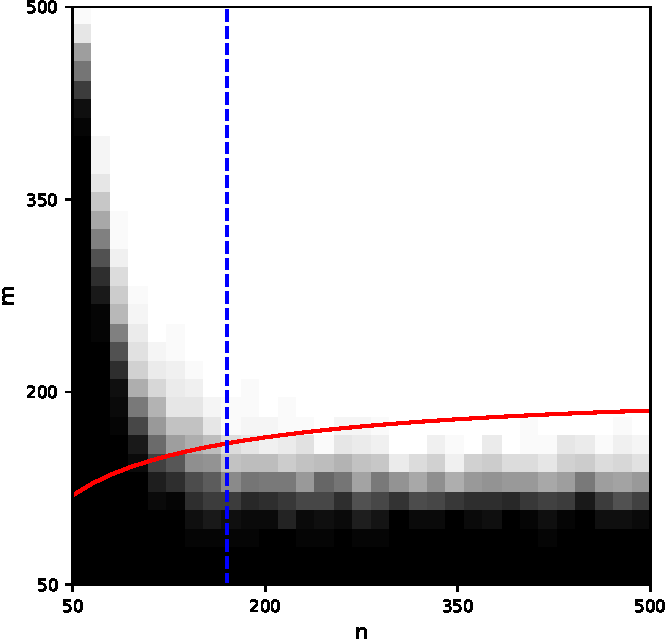
\includegraphics[width=.5\linewidth]{./figures/relation_m_n.pdf}
    \caption{Phase-transition plots for demixing the sum of randomly-rotated sparse signals $\{x\nai\}_{i=1}^k$ from noiseless measurements $b$. The horizontal and vertical axes, respectively, represent the signal dimension $n$ and measurement dimension $m$. The colormap indicates the empirical probability of successful demixing over 50 trials. The red solid curve approximately represents the mapping $\sqrt{m} = \sum_{i=1}^k \sqrt{\delta(\Dscr_i)}$ and the blue dashed line approximately represents the position $\sqrt{n} = \sum_{i=1}^k \sqrt{\delta(\Dscr_i)}$.}
    \label{fig:phase_transition1}
\end{figure}

\subsubsection{Relation between $m$ and $k$}
We also show a phase portrait for the noiseless case that verifies the relationship between number of measurement $m$ and number of signals $k$ stated in \autoref{corollary-stability}. The signal dimension is fixed at $n=1000$ and the sparsity level is fixed at $s=3$. The phase plot is shown in \autoref{fig:phase_transition2}, where the horizontal axis represents the number of signals $k\in\{2, 3, \dots, 10\}$ and the vertical axis represents the number of measurements $m\in\{100, 200, \dots, 1000\}$. All the other settings are the same as stated in \autoref{sec:phase_transition1}. The red line corresponds to $\sqrt{m} = \sum_{i=1}^k \sqrt{\delta(\Dscr_i)}$ and shows that recovery is possible provided the number of measurements scale as $k^2$, when the complexity of all of unknown signals are the same.

\begin{figure}[t]
    \centering\small
    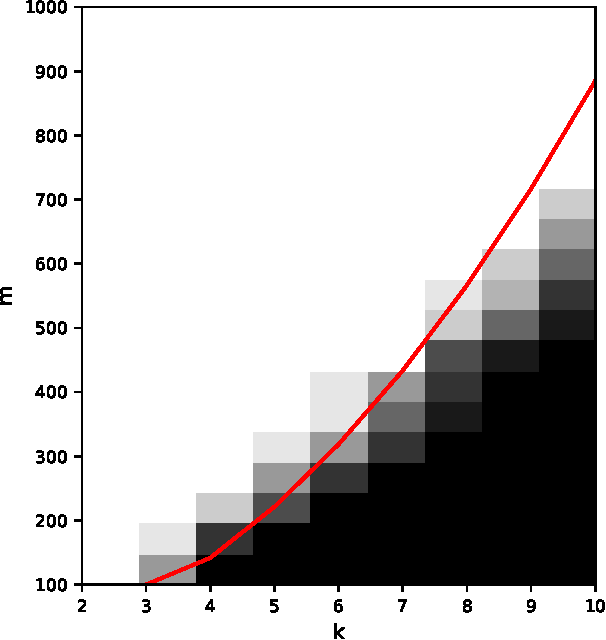
\includegraphics[width=.5\linewidth]{./figures/relation_m_k.pdf}
    \caption{Phase-transition plots for demixing the sum of randomly-rotated sparse signals $\{x\nai\}_{i=1}^k$ from noiseless measurements $b$. The horizontal and vertical axes, respectively, represent the number of signals $k$ and measurement dimension $m$. The colormap indicates the empirical probability of successful demixing over 50 trials. The red solid curve approximately represents the mapping $\sqrt{m} = \sum_{i=1}^k \sqrt{\delta(\Dscr_i)}$.}
    \label{fig:phase_transition2}
\end{figure}

\subsubsection{Relation between maximal absolute error and noise level}
Lastly, we show a plot for the noisy case that verifies the relationship between maximum absolute error $\mathop{\tt maxerr}$ and noise level $\alpha$ stated in \autoref{corollary-stability}. The number of measurement is fixed at $m=125$, the signal dimension is fixed at $n=200$, the number of signals is fixed at $k=3$, and the sparsity level is fixed at $s=5$. The result is shown in \autoref{fig:phase_transition3}, where the horizontal axis represents the noise level $\alpha\in\{0.01, 0.02, \dots, 2\}$ and the vertical axis represents the maximum absolute error $\mathop{\tt maxerr}$. The blue curve corresponds to the mean of $\mathop{\tt maxerr}$ over 50 trials and the yellow shaded area corresponds to the standard deviation. The figure verifies the linear dependence of the recovery error with the noise level, as stated in \autoref{corollary-stability}.

\begin{figure}[t]
    \centering\small
    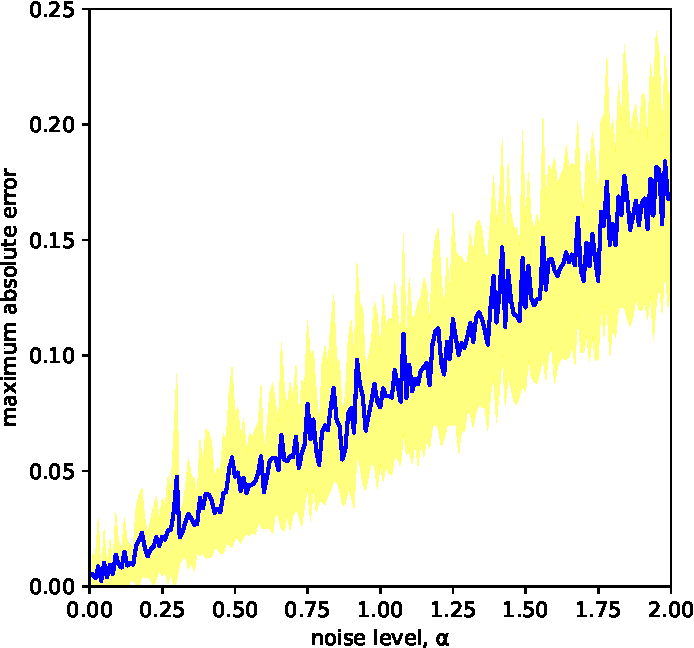
\includegraphics[width=.5\linewidth]{./figures/relation_e_noise.pdf}
    \caption{Error-noise plot for demixing the sum of randomly-rotated sparse signals $\{x\nai\}_{i=1}^k$ from noisy measurements $b$. The horizontal and vertical axes, respectively, represent the noise level $\alpha$ and the maximum absolute error $\mathop{\tt maxerr}$. The blue curve indicates the relationship between the empirical average of $\mathop{\tt maxerr}$ over 50 trials and $\alpha$, and the yellow shaded area indicated the empirical standard deviation. }
    \label{fig:phase_transition3}
\end{figure}


\subsection{Separation of sparse and sparse-in-frequency signals} \label{sec:3-5-2}

\begin{figure}[t]
    \centering
   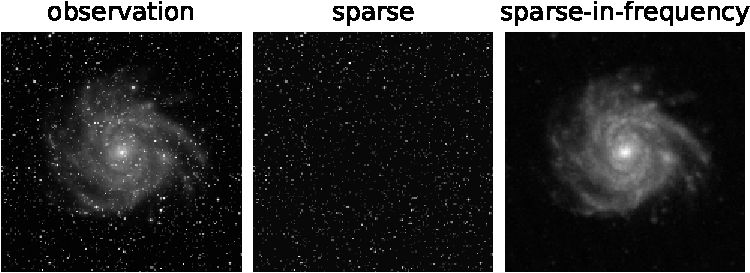
\includegraphics[width=.9\textwidth]{./figures/StarGalaxy.pdf}
    \caption{The star-galaxy separation experiment features two distinct signal components. The image size is $601\times601$ pixels.}
    \label{fig:star_galaxy}
\end{figure}

We reproduce the experiments done by \citet{mccoy2014convexity} on separating an astronomical image into a sparse and a sparse-in-frequency signals. An $n$-vector $x$ is sparse-in-frequency if its discrete cosine transform (DCT) $Dx$ is sparse, where the orthogonal linear map $D:\Re^n\to\Re^n$ encodes the DCT. Define the observations and corresponding atomic sets
\[
  b = x\na_s + x\na_d,
  \quad
  \Ascr_s \coloneqq  \{\pm e_1, \dots, \pm e_n\}, \quad \Ascr_d = D^*\Ascr_s.
\]
The star-galaxy image shown in \autoref{fig:star_galaxy} exemplifies this superposition: the stars are well-represented by sparse matrices in $\Ascr_s$, and the galaxy component is well-represented by sinusoidal elements in $\Ascr_d$. The image size is $601\times601$. The results of the separation are shown in the second two panels of \autoref{fig:star_galaxy}.

\subsection{Sparse and low rank matrix decomposition with structured noise}\label{sec:3-5-3}

In this next example we decompose an image that contains a sparse foreground, a low-rank background, and structured noise. This is an example of sparse principle component analysis~\citep{fazel1998approximations,fhb01,pati1994phase,valiant1977graph}. Typically, the entry-wise 1-norm and the nuclear norm are used to extract from the matrix each of these qualitatively different structures. Here, we treat the noise as its own signal that also needs to be separated. We consider the observations
\[B = X\na_s + X\na_l + X\na_n,\]
where $X\na_s\in\Re^{m\times n}$ is sparse, $X\na_l\in\Re^{m\times n}$ is low-rank matrix, and $X\na_n\in\Re^{m\times n}$ represents structured noise so that $PX\na_nQ$ is sparse, where $P$ and $Q$ are random orthogonal $m$-by-$m$ matrices. Based on the atomic framework, we choose the atomic sets for $X\na_s$, $X\na_l$, and $X\na_n$, respective, as
\begin{align*}
    \Ascr_s &= \{\pm E_{i,j} \mid 1 \leq i \leq m, 1 \leq j \leq n \},
  \\\Ascr_l &= \{uv^\intercal \mid u \in \Re^m,\ v \in \Re^n,\ \|u\|_2=\|v\|_2 = 1\},
  \\\Ascr_n &= P^\intercal\Ascr_s Q^\intercal,
\end{align*}
where $E_{i,j}$ is a $m\times n$ matrix with a single nonzero entry $(i,j)$ with value $1$. 

For the numerical experiment, we consider the noisy chess board in-painting problem. The chess foreground is sparse and the chess board background is low rank. The image size is $596\times596$. The experiment result is shown in~\autoref{fig:chess_board}. 

\begin{figure}[t]
    \centering
    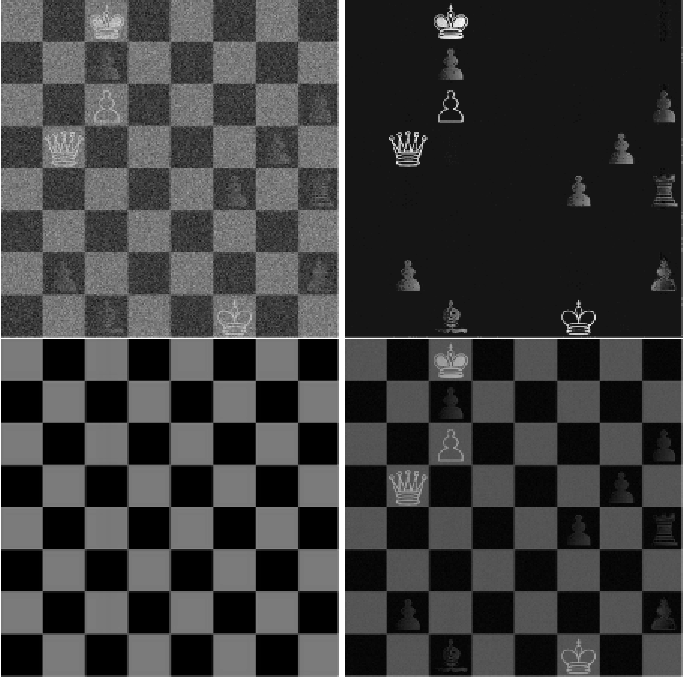
\includegraphics[width=.6\textwidth]{./figures/ChessBoard.pdf}
    \caption{Noisy chess board in-painting experiment. The image size is $596\times596$. Northwest: noisy observations; Northeast: recovered sparse component; Southwest: recovered low rank component; Southeast: denoising result.}
    \label{fig:chess_board}
\end{figure}

\subsection{Multiscale low rank matrix decomposition} \label{sec:3-5-4}

The multiscale low-rank matrix decomposition problem proposed by \citet{ong2016beyond} generalizes the sparse and low-rank matrix decomposition through a block-wise low-rank structure. Let $X$ be an $m \times n$ matrix and $\Pscr$ be a partition of $X$ into multiple blocks. Then $X$ is considered to be block-wise low-rank with respect to $\Pscr$ if all the blocks are low rank. For each block $p\in\Pscr$ with size $m_p \times n_p$, let $X_p$ denote the corresponding part of the matrix $X$ and let $R_p: \Re^{m \times n} \to \Re^{m_p \times n_p}$ denote the linear operator that can extract $X_p$ from $X$, namely $R_p(X) = X_p$. The adjoint operator $R_p^*: \Re^{m_p \times n_p} \to \Re^{m \times n}$ embeds an $m_p \times n_p$ matrix into a $m \times n$ zero matrix. With this operator, 
\begin{equation*}
  X = \sum\limits_{p \in \Pscr} R_p^*(X_p).
\end{equation*}

Each block-wise low-rank signal is represented by a corresponding atomic set. By definition, each block $X_p \in \Re^{m_p \times n_p}$ is low rank, and thus $X_p$ is $\Ascr_p$-sparse, where 
\[
  \Ascr_p = \left\{uv^\intercal \mid u \in \Re^{m_p}, v \in \Re^{n_p}, \|u\| = \|v\| = 1\right\}.
\]
One and Lustig~\cite{ong2016beyond} propose a block-wise nuclear norm and its associated dual norm, respectively, by the functions 
\[
  \|\cdot\|_{\Pscr,1} = \textstyle \sum_{p \in \Pscr} \|R_p(\cdot)\|_1,
  \quad
  \|\cdot\|_{\Pscr,\infty} = \max_{p \in \Pscr} \|R_p(\cdot)\|_{\infty},
\]
where $\|\cdot\|_1$ and $\|\cdot\|_\infty$ are the Schatten 1- and $\infty$-norms of their matrix arguments. It follows that the block-wise norm $\|\cdot\|_{\Pscr,1}$ and dual norm $\|\cdot\|_{\Pscr,\infty}$ are the gauge and support functions, respectively, for the atomic set $\Ascr_\Pscr \coloneqq  \bigcup_{p \in \Pscr} R_p^*\Ascr_p$.

We reproduce the synthetic model described by Ong and Lustig, who construct the superposition $B = \sum_{i = 1}^k X\nai$,
where $X\nai \in \Re^{m \times n}$ is block-wise low rank with respect to the multiscale partitions $\{\Pscr_i\}_{i = 1}^k$. In our experiment, we set $m = n = 64$, $k = 4$, and for each $i\in\irange1k$,
\[m_p = n_p = 4^{i-1}  \quad \forall p \in \Pscr_i.\]
At the lowest scale $i=1$, a block-wise low-rank matrix is a scalar, and so 1-sparse matrices are included with the atomic set $\Ascr_{\Pscr_1}$.  The solutions of the deconvolution procedure \eqref{eq:deconvolution} are shown in~\autoref{fig:multiscale}.

\begin{figure}[t]
    \centering
    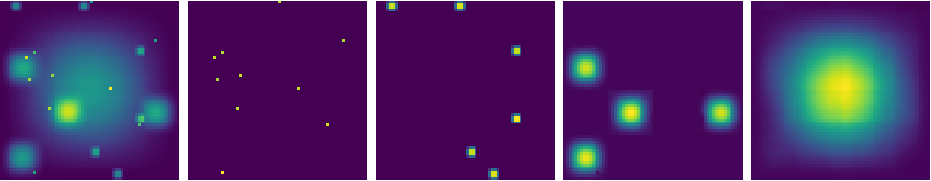
\includegraphics[width=\textwidth]{./figures/Multiscale.pdf}
    \caption{Multiscale low rank matrix decomposition experiment. The matrix size is $64\times64$. From left to right: observations; recovered $\Pscr_i$-block-wise low rank component for $i = 1,\dots,4$. All the blocks in $\Pscr_i$ have the same size $4^{i-1}\times4^{i-1}$ for $i = 1,\dots,4$.}
    \label{fig:multiscale}
\end{figure}






\section{Proofs} \label{sec:3-7}

This section contains proofs for the mathematical statements in this chapter. We begin with several technical results needed for analysis, which describe useful properties of descent cones. Some of these results contain their own intrinsic interest.

\subsection{Lemmas} \label{sec:3-7-1}

\begin{lemma}[Properties of descent cones]\label{prop-descent-cone-properties} Let $\Ascr$, $\Ascr_1$, $\Ascr_2$ be compact sets in $\Re^n$ that contain the origin in their interiors. Fix the vectors $x, x_1, x_2$. The following properties hold.
    \begin{itemize}
     \item[(a)] \label{prop-descent-cone-properties-a}
       A vector $d$ is contained in $\Dscr(\Ascr, x)$ if and only if there is some $\bar\alpha > 0$ such that $\gauge\As(x + \alpha d) \leq \gauge\As(x)$ for all $\alpha \in [0, \bar\alpha]$;
     \item[(b)] \label{prop-descent-cone-properties-b}
       $\Dscr(\tau\Ascr, x) = \Dscr(\Ascr, x)\ \forall\tau > 0$;
     \item[(c)] \label{prop-descent-cone-properties-c}
       $\Dscr(Q\Ascr, Qx) = Q\Dscr(\Ascr, x)$ if $Q\in \SO(n)$;
     \item[(d)] \label{prop-descent-cone-properties-d}
       $\Dscr(\Ascr_1 + \Ascr_2, x_1 + x_2) \subseteq \Dscr(\Ascr_1, x_1) + \Dscr(\Ascr_2, x_2)$ if $\gauge\Aso(x_1) = \gauge\Ast(x_2)$.
     \end{itemize}
\end{lemma} 

\begin{proof}
    \leavevmode
      \begin{itemize}
        \item[(a)] See \citep[Proposition 2.5]{mccoy2014sharp};
        \item[(b)] It follows from the fact that a gauge function is positive homogenous.  
        % \[\Dscr(\tau\Ascr, x) = \cone\set{d \mid \gauge_{\tau\Ascr}(x + d) \leq \gauge_{\tau\Ascr}(x)} = \cone\set{d \mid \gauge_{\Ascr}(x + d) \leq \gauge_{\Ascr}(x)}.\]
        \item[(c)] Because $\gauge_{Q\Ascr}=\gauge_\Ascr(Q^*\cdot)$,
        \begin{align*}
          \Dscr(Q\Ascr, Qx) &= \cone\{d \mid \gauge_{Q\Ascr}(Qx + d) \leq \gauge_{Q\Ascr}(Qx)\}
          \\&= \cone\{d \mid \gauge_{\Ascr}(x + Q^*d) \leq \gauge_{\Ascr}(x)\}
          \\&= Q\Dscr(\Ascr, x).
        \end{align*}
        \item[(d)] 
        For every $d \in \Dscr(\Ascr_1 + \Ascr_2, x_1 + x_2)$, by \autoref{prop-descent-cone-properties-a}(a), there exists $\alpha > 0$ such that  
        \[\gauge\Asum(x_1 + x_2 + \alpha d) \leq \gauge\Asum(x_1 + x_2).\] 
        Then there exists $d_1, d_2$ such that $d_1 + d_2 = \alpha d$ and 
        \[\max\{\gauge\Aso(x_1 + d_1), \gauge\Ast(x_2 + d_2)\} \leq \gauge\Asum(x_1 + x_2).\]
        By the fact that $\gauge\Asum(x_1 + x_2) \leq \max\{\gauge\Aso(x_1), \gauge\Ast(x_2)\}$ and the assumption $\gauge\Aso(x_1) = \gauge\Ast(x_2)$, it follows that $d_i \in \Dscr(\Ascr_i, x_i)$, which implies $\alpha d = d_1 + d_2 \in \Dscr(\Ascr_1, x_1) + \Dscr(\Ascr_2, x_2)$. Thus $d \in \Dscr(\Ascr_1, x_1) + \Dscr(\Ascr_2, x_2)$.
      \end{itemize}
\end{proof}

The Gaussian width of a set $T \subset \Re^n$ is defined as
\[\omega(T) = \mE_{g} \sup\{ \ip{g}{y} | y\in T\},\]
where the expectation is taken with respect to the standard Gaussian $\Nscr(0,I_n)$. 
The following lemma summarizes the main properties that we use regarding the relationship between the conic summaries $\delta$ and $\omega$.

\begin{lemma}[Properties of conic statistical summaries]\label{prop:stat_dim}
    Let $\Kscr$ be a closed and convex cones in $\Re^n$ and let $Q\in\SO(n)$. Then the following properties hold. 
    \begin{itemize}
      \item[(a)] \label{prop:stat_dim_a} $\delta(Q\Kscr) = \delta(\Kscr)$;
      \item[(b)] \label{prop:stat_dim_b} $\delta(\Kscr) = \mE_g \left[\sup\{ \ip{g}{y} | y\in\Kscr\cap\mB^n\}^2\right]$;
      \item[(c)] \label{prop:stat_dim_c} $\omega(\Kscr\cap\mB^n)^2 \leq \delta(\Kscr)$.
    \end{itemize}
\end{lemma}

\begin{proof} 
    See \citep[Proposition~3.1(6) and Proposition~3.1(5)]{amelunxen2014living}, respectively, for (a) and (b). 
    \begin{itemize}
      \item[(c)] Indeed, we know that,
      \begin{align*}
        \omega(\Kscr\cap\mB^n)^2 &= \left[\mE_{g} \sup\{ \ip{g}{y} | y\in \Kscr\cap\mB^n\}\right]^2
        \\&\leq \mE_{g} \left[\sup\{ \ip{g}{y} | y\in \Kscr\cap\mB^n\}^2\right]
        \\&= \delta(\Kscr),
      \end{align*}
      where the first equality follows from the definition of gaussian with, the first inequality follows from the fact that $\mE(X)^2 \leq \mE(X)^2$ for any random variable $X$, and the last equality follows from \autoref{prop:stat_dim_b}(b). 
    \end{itemize}
\end{proof}

Our next lemma shows that if the angle between two cones is bounded, then the norms of individual vectors are bounded by the norm of their sum.

\begin{lemma}\label{lemma:bound_norm}
    Let $\Kscr_1$ and $\Kscr_2$ be two closed convex cones in $\Re^n$. If $\cos\angle(-\Kscr_1, \Kscr_2) \leq 1 - \beta$ for some $\beta \in (0, 1]$, then for any $u \in \Kscr_1$ and $v \in \Kscr_2$, 
    \[\max\{\|u\|, \|v\|\} \leq \frac{1}{\sqrt{\beta}}\|u + v\|.\]
\end{lemma}

\begin{proof}
    By expanding the norm square of $u + v$ we can get that 
      \begin{align*}
        \|u + v\|^2 &= \|u\|^2 + \|v\|^2 - 2\ip{-u}{v}
        \\&= \|u\|^2 + \|v\|^2 - 2\cos(\angle(-u, v))\|u\|\|v\|
        \\&\geq \|u\|^2 + \|v\|^2 - 2(1-\beta)\|u\|\|v\|
        \\&= \beta(\|u\|^2 + \|v\|^2) + (1-\beta)(\|u\| - \|v\|)^2
        \\&\geq \beta\max\{\|u\|^2, \|v\|^2\},
      \end{align*}
    where the first inequality follows from the definition of the cosine of the angle between two cones. 
\end{proof}

Our next lemma is a technical lemma for the expectation.

\begin{lemma}\label{lemma:expectation}
    Let $X$ and $Y$ be nonnegative random variables, then we have 
    \[\mE[(X+Y)^2] \leq \left( \sqrt{\mE[X^2]} + \sqrt{\mE[Y^2]} \right)^2.\]
\end{lemma}

\begin{proof}
    By expanding the right hand side, we can get
    \begin{align*}
      \left( \sqrt{\mE[X^2]} + \sqrt{\mE[Y^2]} \right)^2 &= \mE[X^2] + \mE[Y^2] + 2\sqrt{\mE[X^2]\mE[Y^2]}
      \\&\geq \mE[X^2] + \mE[Y^2] + 2\mE[XY]
      \\&= \mE[(X+Y)^2],
    \end{align*}
    where the inequality follows from the Cauchy–Schwarz inequality.
\end{proof}

\subsection{Proof for \titlelink{\autoref{thm-stability}}} \label{sec:proof-thm-stability}
For each $i\in\irange1k$, let $\epsilon_i \coloneqq  x_i^* - x\nai$ and $\epsilon_{-i} : = \sum_{j \neq i}\epsilon_j$. By the definition of descent cone,
$\epsilon_i \in \Dscr(\Ascr_i, x\nai$).
Because $\{(x\nai, \Ascr_i)\}_{i=1}^k$ are $\beta$-incoherent for some $\beta\in(0,1]$, by~\autoref{def:incoherence},
\[\cos\angle\left(-\epsilon_i, \epsilon_{-i}\right) \leq 1 - \beta.\]
By \autoref{lemma:bound_norm}, it follows that
\[ \left\|\epsilon_i + \epsilon_{-i}\right\| \geq \sqrt{\beta}\|\epsilon_i\|.\]
The desired result follows.

\subsection{Proof for \titlelink{\autoref{prop:bound_sta_dim}}} \label{sec:proof-bound_sta_dim}
In this proof, we define $\Kscr_{i, \beta} =  \Kscr_i \cap \tfrac{1}{\sqrt{\beta}} \mB^n$ and $f_{i, \beta}(g) = \sup\{ \ip{g}{u} | u \in \Kscr_{i, \beta}\}$ for $i = 1, 2$. By \autoref{prop:stat_dim_b}, we know that the statistical dimension can be expressed as
\begin{align*}
  \delta(\Kscr_1 + \Kscr_2) &= \mE_g \left[\sup\{ \ip{g}{y} | y\in(\Kscr_1 + \Kscr_2)\cap\mB^n\}^2 \right]
  \\&= \mE_g \left[\sup\{ \ip{g}{u + v} | u \in \Kscr_1, v \in \Kscr_2, \|u + v\| \leq 1 \}^2\right]
  \\&\leq \mE_g \left[\sup\{ \ip{g}{u + v} | u \in \Kscr_{1, \beta}, v \in \Kscr_{2, \beta} \}^2\right]
  \\&= \mE_g \left[ \left(\sup\{ \ip{g}{u} | u \in \Kscr_{1, \beta}\} + \sup\{ \ip{g}{v} | v \in \Kscr_{2, \beta}\} \right)^2 \right]
  \\&\leq \left( \sqrt{ \mE_g \left[ f_{1, \beta}(g)^2 \right]} + \sqrt{ \mE_g \left[ f_{2, \beta}(g)^2 \right]} \right)^2
  % \\&= \left( \tfrac{1}{\sqrt{\beta}} \sqrt{ \mE_g \left[ \sup\set{ \ip{g}{u} | u \in \Kscr_1 \cap \mB^n}^2 \right]} + \tfrac{1}{\sqrt{\beta}} \sqrt{ \mE_g \left[ \sup\set{ \ip{g}{v} | v \in \Kscr_2 \mB^n}^2 \right]} \right)^2
  \\&= \tfrac{1}{\beta}\left(\sqrt{\delta(\Kscr_1)} + \sqrt{\delta(\Kscr_2)} \right)^2
\end{align*}
where the first inequality follows from \autoref{lemma:bound_norm} and the fact that the supremum is always nonnegative, and the second inequality follows from \autoref{lemma:expectation}. 

\subsection{Proof for \titlelink{\autoref{coro:bound_sta_dim}}} \label{sec:proof-coro-bound_sta_dim}
Throught this proof, for all $i\in1:k$, we define $\Dscr_i = \Dscr(\Ascr_i, x\nai)$, $\delta_i = \delta(\Dscr_i)$ and $\delta_{1:i} = \delta(\sum_{j=1}^i\Dscr_i)$. By \autoref{assume-blanket} and \autoref{prop-descent-cone-properties-d}, we know that $\Dscr\subs \subseteq \sum_{i=1}^k \Dscr_i$, and it follows that $\delta(\Dscr\subs)\leq\delta_{1:k}$. So we only need to give an upper bound for $\delta_{1:k}$. Since $\cos\angle\left({-\Dscr_k},\, \sum_{i=1}^{k-1}\Dscr_i\right)\leq 1 - \beta$, by \autoref{prop:bound_sta_dim}, it follows that 
\begin{equation} \label{eq:111}
  \sqrt{\delta_{1:k}} \leq \beta^{-\tfrac{1}{2}}\left(\sqrt{\delta_{1:(k-1)}} + \sqrt{\delta_k}\right).
\end{equation}
Since $\sum_{i=1}^{k-2}\Dscr_i \subseteq \sum_{j\neq(k-1)}\Dscr_j$, it follows that $\cos\angle\left({-\Dscr_{k-1}},\, \sum_{i=1}^{k-2}\Dscr_i\right)\leq  1 - \beta$. By \autoref{prop:bound_sta_dim}, we have 
\begin{equation} \label{eq:112}
  \sqrt{\delta_{1:(k-1)}} \leq \beta^{-\tfrac{1}{2}}\left(\sqrt{\delta_{1:(k-2)}} + \sqrt{\delta_{k-1}}\right).
\end{equation}
Combining \eqref{eq:111} and \eqref{eq:112}, we know that 
\[\sqrt{\delta_{1:k}} \leq \beta^{-\tfrac{2}{2}}\left(\sqrt{\delta_{1:(k-2)}} + \sqrt{\delta_{k-1}} + \sqrt{\delta_k}\right).\]
Repeating this process, we can conclude that 
\[\sqrt{\delta_{1:k}} \leq \beta^{-\tfrac{k-1}{2}}\sum_{i=1}^k\sqrt{\delta_i}.\]

\subsection{Proof for \titlelink{\autoref{prop-angle-cones}}}\label{sec:proof-prop-angle-cones}
Throught this proof, we define the following notations:
\begin{itemize} 
  \item $\overline\Kscr_i:=\Kscr_i\cap\mS^{n-1}$ for $i=1,2$;
  \item $\widehat\Kscr_i:=\Kscr_i\cap\mB^n$ for $i=1,2$;
  \item $f(W\in\Re^{n\times n}) = \sup\{\ip{x}{Wy} \mid x \in \overline\Kscr_1, y \in\overline\Kscr_2\}$;
  \item $\hat f(W\in\Re^{n\times n}) = \sup\{\ip{x}{Wy} \mid x \in \widehat\Kscr_1, y \in\widehat\Kscr_2\}$;
  \item $\Oscr_n = \{Q\in\Re^{n\times n}: Q^TQ = I_n\}$;
  \item $\Sscr\Oscr_{n, +} = \{Q\in\Oscr_n: \det(Q) = 1\}$;
  \item $\Sscr\Oscr_{n, -} = \{Q\in\Oscr_n: \det(Q) = -1\}$.
\end{itemize} 

Our proof consists of three steps. 

\paragraph{First step: show that both $f$ and $\hat f$ are convex and $1$-Lipschitz functions.} First, we show that both $f$ and $\hat f$ are convex. 
For any $W_1, W_2 \in \Re^{n\times n}$ and any $t \in [0,1]$, 
\begin{align*}
  &f(tW_1 + (1-t)W_2) 
  \\&= \sup\{\ip{x}{(tW_1 + (1-t)W_2)y} \mid x \in \overline\Kscr_1, y \in\overline\Kscr_2\}
  \\&= \sup\{\ip{x}{tW_1y} + \ip{x}{(1-t)W_2y} \mid x \in \overline\Kscr_1, y \in\overline\Kscr_2\}
  \\&\leq tf(W_1) + (1-t)f(W_2).
\end{align*}
So $f$ is convex. The same reason holds for $\hat f$, and thus $\hat f$ is also convex. 
Next, by \citep[Lemma~2.6]{shalev2011online}, in order to show that both $f$ and $\hat f$ are $1$-Lipschitz, we only need to show that the norm of any subgradient of $f$ or $\hat f$ is bounded by $1$. By \citep[Theorem~D.4.4.2]{hiriart-urruty01}, we know that for any $W \in \Re^{n\times n}$, 
\begin{align*}
  \partial f(W) &= \conv\{xy^T \mid x \in \overline\Kscr_1, y \in\overline\Kscr_2, \ip{x}{Wy} = f(W)\},
  \\ \partial \hat f(W) &= \conv\{xy^T \mid x \in \widehat\Kscr_1, y \in\widehat\Kscr_2, \ip{x}{Wy} = f(W)\}.
\end{align*}
Since $\|x\| \leq 1$ and $\|y\| \leq 1$, it is easy to verify that for any $W\in\Re^{n\times n}$ and for any $Z \in \partial f(W) \cup \partial \hat f(W)$, 
\[\|Z\|_F \leq 1,\]
where $\|\cdot\|_F$ is the Frobenius norm. Therefore, we can conclude that both $f$ and $\hat f$ are $1$-Lipschitz functions.


\paragraph{Second step: bound $\mE_{Q \sim \uniform(\Sscr\Oscr_{n, +})}\left[f(Q)\right]$.} 
First, we give the bound on 
\[\mE_{Q \sim \uniform(\Oscr_n)}\left[\hat f(Q)\right].\] 
From the first step, we know that $\hat f$ is convex. Then by the comparison principle developed by Tropp; see \citep[Theorem~5 and Lemma~8]{tropp2012comparison}, we can conclude that 
\begin{equation} \label{eq:help1}
  \mE_{Q \sim \uniform(\Oscr_n)}\left[\hat f(Q)\right] \leq \tfrac{1.5}{\sqrt{n}}\mE_{G\sim\Nscr(0, I_n)}\left[\hat f(G)\right],
\end{equation}
Next, we give the bound on $\mE_{Q \sim \uniform(\Sscr\Oscr_{n, +})}\left[\hat f(Q)\right]$. By expanding the uniform distribution over $\Oscr_n$, we can get
\begin{align*}
  &\mE_{Q \sim \uniform(\Oscr_n)}\left[\hat f(Q)\right] 
  \\&= \tfrac{1}{2}\mE_{Q \sim \uniform(\Sscr\Oscr_{n, +})}\left[\hat f(Q)\right] + \tfrac{1}{2}\mE_{Q \sim \uniform(\Sscr\Oscr_{n, -})}\left[\hat f(Q)\right]
  \\&\geq \tfrac{1}{2}\mE_{Q \sim \uniform(\Sscr\Oscr_{n, +})}\left[\hat f(Q)\right],
\end{align*}
where the inequality follows from the fact that $\hat f$ is non-negative. Combine this result with \eqref{eq:help1}, we can conclude that 
\begin{equation} \label{eq:help2}
  \mE_{Q \sim \uniform(\Sscr\Oscr_{n, +})}\left[\hat f(Q)\right] \leq \tfrac{3}{\sqrt{n}}\mE_{G\sim\Nscr(0, I_n)}\left[\hat f(G)\right].
\end{equation}
Then, by the Gaussian Chevet’s inequality; see\citep[Exercise~8.7.4]{vershynin2018high}, we know that 
\begin{equation} \label{eq:help3}
  \mE_{G\sim\Nscr(0, I_n)}\left[\hat f(G)\right] \leq \omega(\widehat\Kscr_1) + \omega(\widehat\Kscr_2) \leq \sqrt{\delta(\Kscr_1)} + \sqrt{\delta(\Kscr_2)},
\end{equation}
where the second inequality follows from \autoref{prop:stat_dim_c}. Combine \eqref{eq:help2} and \eqref{eq:help3}, we can get
\begin{equation} \label{eq:help4}
  \mE_{Q \sim \uniform(\Sscr\Oscr_{n, +})}\left[\hat f(Q)\right] \leq \tfrac{3}{\sqrt{n}}\left( \sqrt{\delta(\Kscr_1)} + \sqrt{\delta(\Kscr_2)} \right).
\end{equation}
Finally, by the fact that $f \leq \hat f$ and \eqref{eq:help4}, we can conclude that 
\begin{equation} \label{eq:help5}
  \mE_{Q \sim \uniform(\Sscr\Oscr_{n, +})}\left[f(Q)\right] \leq \tfrac{3}{\sqrt{n}}\left( \sqrt{\delta(\Kscr_1)} + \sqrt{\delta(\Kscr_2)} \right).
\end{equation}

\paragraph{Third step: concentration bound for $f(Q)$.}
From step 1, we know that $f$ is $1$-Lipschitz. For clearness, we denote $\mP_{Q \sim \uniform(\Sscr\Oscr_{n, +})}$ and $\mE_{Q \sim \uniform(\Sscr\Oscr_{n, +})}$ as $\mP_Q$ and $\mE_Q$. By the concentration bounds of Lipschitz functions over the special orthogonal group develop by Meckes; see \citep[Theorem~5.5 and Theorem~5.16]{meckes2019random}, we can get that for every $t\geq0$,
\[\mP_Q\left[f(Q) \geq \mE_Q[f(Q)] + t\right] \leq \exp(-\tfrac{n-2}{8}t^2).\]
Note that a similar result can be obtained from \citep[Theorem~5.2.7]{vershynin2018high}.
Combining with \eqref{eq:help5}, we can conclude that for every $t\geq0$,
\[\mP_Q\left[f(Q) \geq  \tfrac{3}{\sqrt{n}}\left( \sqrt{\delta(\Kscr_1)} + \sqrt{\delta(\Kscr_2)} \right) + t\right] \leq \exp(-\tfrac{n-2}{8}t^2).\]

\subsection{Lemmas needed for the proof of \titlelink{\autoref{thm:Incoherence}}} \label{sec:prob_bounds}
In this section, we present two lemmas that are needed for the proof of \autoref{thm:Incoherence}. These two lemmas provide probabilistic bound on the statistical dimension of sum of randomly rotated cones. 

The next lemma provides a probabilistic bound on the statistical dimension of the sum of two cones. 
\begin{lemma}[Probabilistic bound on statistical dimension under random rotation] \label{prop-bound-sta-dim}
   Let $\Kscr_1$ and $\Kscr_2$ be two closed convex cones in $\Re^n$. Then 
 \begin{align*}
   \mP\bigg[\sqrt{\delta(\Kscr_1 + Q\Kscr_2)} &\leq \tfrac{1}{\sqrt{\beta(t)}}\left(\sqrt{\delta(\Kscr_1)} + \sqrt{\delta(\Kscr_2)} \right) \bigg]
   \\&\geq 1 - \exp(-\tfrac{n-2}{8}t^2)
   \\\text{with} \beta(t) &= 1 - \tfrac{3}{\sqrt{n}}\left(\sqrt{\delta(\Kscr_1)} + \sqrt{\delta(\Kscr_2)}\right) - t ,
 \end{align*}
   where $Q$ is drawn uniformly at random from $\SO(n)$.
\end{lemma}

\begin{proof}
    By \autoref{prop:bound_sta_dim} and \autoref{prop-angle-cones}.
\end{proof}

Our next lemma extends \autoref{prop-bound-sta-dim} to arbitrary number of cones. 
\begin{lemma} \label{prop:bound-sum-sta-dim}
   Let $\Kscr_1, \dots, \Kscr_p$ be closed convex cones in $\Re^n$ and let $Q_1, \dots, Q_p$ be i.i.d. matrices uniformly drawn from $\SO(n)$. If $\sum_{i=1}^p \sqrt{\delta(\Kscr_i)} \leq \left(1 - 4^{- \tfrac{1}{p-1} } - t\right)\sqrt{n} / 6$ for some $t > 0$, then 
   \begin{equation*}
   \mP\left[ \sqrt{\delta\left(\sum_{i=1}^pQ_i\Kscr_i\right)} \leq 2\sum_{i=1}^p \sqrt{\delta(\Kscr_i)}\right] \geq 1 - (p-1)\exp(-\tfrac{n-2}{8}t^2).
   \end{equation*}
\end{lemma}

\begin{proof}
    Throughout this proof, we define the following notations:
    \begin{itemize}
      \item $\delta_i = \delta(\Kscr_i)$, for all $i\in1:p$;
      \item $\delta_{1:i} = \delta\left(\sum_{j=1}^iQ_j\Kscr_j\right)$, for all $i\in1:p$;
      \item For each $i\in2:p$, define the event 
    \begin{align*}
      E_i(t) &= \left\{ \sqrt{\delta_{1:i}} \leq \tfrac{1}{\sqrt{\beta_i(t)}} \left( \sqrt{\delta_{1:(i-1)}} + \sqrt{\delta_i}\right)\right\}
      \\\text{with} \beta_i(t) &= 1 - \tfrac{3}{\sqrt{n}}\left( \sqrt{\delta_{1:(i-1)}} + \sqrt{\delta_i}\right) - t.
    \end{align*}
    \end{itemize}
    
    Our proof consists of three steps.
    
    \paragraph{Step 1:} bound the probability of $E_2(t)\land\cdots\land E_p(t)$.
    Denote the indicator random variable for $E_i(t)$ by $\mathbbm{1}_{E_i(t)}$, which evaluates to $1$ if $E_i(t)$ occurs and otherwise evaluates to $0$. Then for each $i\in2:p$, we have
    \begin{align*}
      \mP(E_i(t)) &= \mE(\mathbbm{1}_{E_i(t)})
      \\&= \mE_{\{Q_j\}_{j=1}^{i-1}} \left[ \mE\left(\mathbbm{1}_{E_i(t)} \mid \{Q_j\}_{j=1}^{i-1}\right)\right]
      \\&\geq \mE_{\{Q_j\}_{j=1}^{i-1}} \left[ 1 - \exp(-\tfrac{n-2}{8}t^2) \right]
      \\&= 1 - \exp(-\tfrac{n-2}{8}t^2),
    \end{align*}
    where the inequality follows from \autoref{prop-bound-sta-dim} and the assumption that $Q_i$ are all independent. Extending the bound on $\mP(E_i(t))$ to all $i\in\irange2p$ via the union bound, we have
    \[
      \mP(E_2(t) \land\cdots\land E_p(t))
      \geq 1 - (p-1)\exp(-\tfrac{n-2}{8}t^2).\]
    
    \paragraph{Step 2:} show that $E_2(t) \land\cdots\land E_p(t)$ implies bound on \[\sqrt{\delta_{1:p}}\leq\tfrac{1}{\sqrt{\beta_2(t)\dots\beta_p(t)}}\sum_{i=1}^p\sqrt{\delta_i}.\] Indeed, we have 
    \begin{align*}
      \sqrt{\delta_{1:p}} &\leq \tfrac{1}{\sqrt{\beta_p(t)}}\left( \sqrt{\delta_{1:(p-1)}} + \sqrt{\delta_p}\right)
      \\&\leq \tfrac{1}{\sqrt{\beta_p(t)}}\left( \tfrac{1}{\sqrt{\beta_{p-1}(t)}}\left( \sqrt{\delta_{1:(p-2)}} + \sqrt{\delta_{p-1}}\right) + \sqrt{\delta_p}\right)
      \\&\leq \tfrac{1}{\sqrt{\beta_p(t)\beta_{p-1}(t)}}\left( \sqrt{\delta_{1:(p-2)}} + \sqrt{\delta_{p-1}} + \sqrt{\delta_p}\right)
      \\&\vdots
      \\&\leq \tfrac{1}{\sqrt{\beta_2(t)\dots\beta_i(t)}}\sum_{j=1}^i\sqrt{\delta_j}.
    \end{align*}
    
    \paragraph{Step 3:} show that $E_2(t) \land\cdots\land E_p(t)$ and the assumption \[\sum_{i=1}^p \sqrt{\delta(\Kscr_i)} \leq \left(1 - 4^{- \tfrac{1}{p-1} } - t\right)\sqrt{n} / 6\] implies that $\beta_i(t) \geq 4^{-\tfrac{1}{k-1} }$ for $i\in2:p$. We prove this by induction on $i$. First we show that $\beta_2(t) \geq 4^{-\tfrac{1}{k-1} }$. Indeed, we have 
    \begin{align*}
      \beta_2(t) &= 1 - \tfrac{3}{\sqrt{n}}\left( \sqrt{\delta_1} + \sqrt{\delta_2}\right) - t
      \\&\geq 1 - \tfrac{3}{\sqrt{n}}\tfrac{ \left(1 - 4^{- \tfrac{1}{k-1} } - t\right)\sqrt{n} }{6} - t
      \geq  4^{-\tfrac{1}{k-1} }.
    \end{align*}
     Next for any $i\in3:k$, we assume that $\beta_j(t) \geq 4^{-\tfrac{1}{k-1} }$ for all $2\leq j \leq (i-1)$, then we have 
    \begin{align*}
      \beta_i(t) &=  1 - \tfrac{3}{\sqrt{n}}\left( \sqrt{\delta_{1:(i-1)}} + \sqrt{\delta_i}\right) - t
      \\&\geq 1 - \tfrac{3}{\sqrt{n}} \tfrac{1}{\sqrt{\beta_2(t)\dots\beta_{i-1}(t)}}\sum_{j=1}^{i}\sqrt{\delta_j} - t
      \\&\geq 1 - \tfrac{3}{\sqrt{n}} 2^{ \tfrac{i-2}{k-1} } \tfrac{ \left(1 - 4^{- \tfrac{1}{k-1} } - t\right)\sqrt{n} }{6} - t
      \geq 4^{- \tfrac{1}{k-1} }.
    \end{align*}
    
    Finally, combining all three steps, we can conclude that 
    \begin{equation*}
      \mP\left[ \sqrt{\delta\left(\sum_{i=1}^pQ_i\Kscr_i\right)} \leq 2\sum_{i=1}^p \sqrt{\delta(\Kscr_i)}\right] \geq 1 - (p-1)\exp(-\tfrac{n-2}{8}t^2).
    \end{equation*}
\end{proof}

\subsection{Proof for \titlelink{\autoref{thm:Incoherence}}} \label{sec:proof-thm:Incoherence}

Throughout this proof, we define the following notations for all $i\in1:k$:
\begin{itemize} 
  \item $\Dscr_i = \Dscr(\Ascr_i, x\nai)$;
  \item $\hat \Dscr_i =  \Dscr(\hat \Ascr_i, \hat x\nai)$;
  \item $\delta_i = \delta(\Dscr_i)$;
  \item $\delta_{1:i} = \delta\left(\sum_{j=1}^i\Dscr_i\right)$;
  \item $\delta_{-i} = \delta\left(\sum_{j\neq i}\Dscr_j\right)$.
\end{itemize} 
By~\autoref{prop-descent-cone-properties-c}, for all $i\in1:k$, we have
\[\Dscr_i = \Dscr(Q_i \hat \Ascr_i, Q_i \hat x\nai) = Q_i\hat\Dscr_i.\]
Then it follows from \autoref{prop:stat_dim_a} that
\[\delta(\hat \Dscr_i) = \delta(Q_i^T \Dscr_i) = \delta_i.\]
For all $i\in\irange1k$, define 
\begin{itemize}
  \item $\hat \Dscr_i\coloneqq  \Dscr(\hat \Ascr_i, \hat x\nai)$;
  \item $\delta_i = \delta(\Dscr_i)$;
  \item $\delta_{-i} = \delta\left(\sum_{j\neq i}\Dscr_j\right)$
\end{itemize}
First, fix $t >0$, for each $i\in\irange1k$, define the event
\[
E_i(t) =  \left \{ \cos\angle\left(-\Dscr_i, \sum_{j \neq i}\Dscr_j\right) \leq \tfrac{3}{\sqrt{n}}\left(\sqrt{\delta_i} + \sqrt{\delta_{-i}}\right) + t \right\}.
\] 
Denote the indicator random variable for $E_i(t)$ by $\mathbbm{1}_{E_i(t)}$, which evaluates to $1$ if $E_i(t)$ occurs and otherwise evaluates to $0$. Then, the following chain of inequalities gives the upper bound for the probability of the event $E_i(t)$:
\begin{align} \label{eq:123}
  \begin{split}
\mP (E_i(t)) 
  &= \mE (\mathbbm{1}_{E_i(t)})
\\&= \mE_{\{Q_j\}_{j\ne i}} \mE\left[\mathbbm{1}_{E_i(t)} \bigm\vert Q_j\ \forall j\ne i \right]
\\&\geq \mE_{\{Q_j\}_{j\ne i}} [ 1 - \exp(-\tfrac{n-2}{8}t^2) ]
\\&= 1 - \exp(-\tfrac{n-2}{8}t^2),
\end{split}
\end{align}
where the inequality follows from \autoref{prop-angle-cones}. 

Next, by \autoref{prop:bound-sum-sta-dim}, we know that 
\begin{equation}\label{eq:223}
  \mP\left[ \sqrt{\delta_{-i}} \leq 2\sum_{j\neq i} \sqrt{\delta_j}\right] \geq 1 - (k-2)\exp(-\tfrac{n-2}{8}t^2).
\end{equation}


Thirdly, for each $i\in\irange1k$, define the event, 
\[
\hat E_i(t) =  \left \{ \cos\angle\left(-\Dscr_i, \sum_{j \neq i}\Dscr_j\right) \leq \tfrac{6}{\sqrt{n}}\sum_{i=1}^k\sqrt{\delta_i} + t\right \}.
\]
By combining \eqref{eq:123} and \eqref{eq:223} together, we can conclude that 
\[\mP(\hat E_i(t)) \geq 1 - (k-1)\exp(-\tfrac{n-2}{8}t^2).\]
Extend the bound on $\mP(\hat E_i(t))$ to all $i\in\irange1k$ via the union bound:
\[\mP(\hat E_1\land\cdots\land \hat E_k) \geq 1 - k(k-1)\exp(-\tfrac{n-2}{8}t^2).\]

Finally, by our assumption
\[\sum_{i=1}^k \sqrt{\delta(\Dscr_i)} \leq \left(1 - 4^{- \tfrac{1}{k-1} } - t\right)\sqrt{n} / 6,\] it follows that 
\[\tfrac{6}{\sqrt{n}}\sum_{i=1}^k\sqrt{\delta_i} + t \leq 1 - 4^{- \tfrac{1}{k-1} }.\]
Therefore, we can conclude that the rotated pairs $\{(x\nai,\Ascr_i)\}_{i=1}^k$ are $4^{- \tfrac{1}{k-1} }$-incoherent with probability at least $1 - k(k-1)\exp(-\tfrac{n-2}{8}t^2)$.










